\documentclass[12pt,letterpaper]{article}
\usepackage{geometry} % see geometry.pdf on how to lay out the page. There's lots.
%\geometry{a4paper} % or letter or a5paper or ... etc
% \geometry{landscape} % rotated page geometry

%% LaTeX - Article customise

%%% PACKAGES
\usepackage{booktabs} % for much better looking tables
\usepackage{array} % for better arrays (eg matrices) in maths
\usepackage{paralist} % very flexible & customisable lists (eg. enumerate/itemize, etc.)
\usepackage{verbatim} % adds environment for commenting out blocks of text & for better verbatim
\usepackage{subfigure} % make it possible to include more than one captioned figure/table in a single float
% These packages are all incorporated in the memoir class to one degree or another...

%%% PAGE DIMENSIONS
\usepackage{geometry} % to change the page dimensions
%\geometry{margins=2cm} % for example, change the margins to 2 inches all round
%\geometry{landscape} % set up the page for landscape
% read geometry.pdf for detailed page layout information

%%% HEADERS & FOOTERS
\usepackage{fancyhdr} % This should be set AFTER setting up the page geometry
\pagestyle{fancy} % options: empty , plain , fancy
\renewcommand{\headrulewidth}{0pt} % customise the layout...
\lhead{}\chead{}\rhead{}
\lfoot{}\cfoot{\thepage}\rfoot{}

%%%% SECTION TITLE APPEARANCE
%\usepackage{sectsty}
%\allsectionsfont{\sffamily\mdseries\upshape} % (See the fntguide.pdf for font help)
%% (This matches ConTeXt defaults)

%% LaTeX Preamble - Common packages

\usepackage[utf8]{inputenc} % Any characters can be typed directly from the keyboard, eg éçñ
\usepackage{textcomp} % provide lots of new symbols
\usepackage{graphicx}  % Add graphics capabilities
%\usepackage{epstopdf} % to include .eps graphics files with pdfLaTeX
\usepackage{flafter}  % Don't place floats before their definition
%\usepackage{topcapt}   % Define \topcation for placing captions above tables (not in gwTeX)
\usepackage{natbib} % use author/date bibliographic citations

\usepackage{amsmath,amssymb}  % Better maths support & more symbols
\usepackage{bm}  % Define \bm{} to use bold math fonts

\usepackage[pdftex,bookmarks,colorlinks,breaklinks]{hyperref}  % PDF hyperlinks, with coloured links
%\definecolor{dullmagenta}{rgb}{0.4,0,0.4}   % #660066
%\definecolor{darkblue}{rgb}{0,0,0.4}
%\hypersetup{linkcolor=red,citecolor=blue,filecolor=dullmagenta,urlcolor=darkblue} % coloured links
%%\hypersetup{linkcolor=black,citecolor=black,filecolor=black,urlcolor=black} % black links, for printed output

\usepackage{memhfixc}  % remove conflict between the memoir class & hyperref
% \usepackage[activate]{pdfcprot}  % Turn on margin kerning (not in gwTeX)
\usepackage{pdfsync}  % enable tex source and pdf output syncronicity

% Defining Itemized List Levels
\renewcommand{\labelitemi}{$-$}
%\renewcommand{\labelitemii}{$\cdot$}
%\renewcommand{\labelitemiii}{$\diamond$}
%\renewcommand{\labelitemiv}{$\ast$}

% Better margins
\usepackage{fullpage}

% Matlab code includer
% load package with ``framed'' and ``numbered'' option.
\usepackage[framed,numbered,autolinebreaks,useliterate]{mcode}

%%% BEGIN DOCUMENT
\begin{document}

% Maybe \noindent

\begin{center}
\huge
Scaling Analysis for Rigid Body Simulations\\
\normalsize
\vspace{0.1in}
Andrew P. (Drew) Sabelhaus\\
apsabelhaus@berkeley.edu \\
Started 14 July 2014 \\
Current as of 8 Jan 2015
\end{center}

%\vspace{-1em}

This short white paper illustrates the scaling analysis that needs to be done on an rigid body simulation system, such as the NASA Tensegrity Robotics Toolkit (NTRT or its C++ library, NTRTsim) and the Bullet Physics system.
This work is designed to convince NTRT/Bullet users that care must be taken for scaling techniques, moreso than occurs on the Bullet Physics forums or wiki.
In particular, simple scalings work in some circumstances with certain types of simulated parameters, but may have to be modified elsewhere (see: scaling of forces, scaling of angular vs. longitudinal spring constants.)
First, we introduce a simple example system for analysis, then do the nondimensionalization of parameters, and evaluate which scalings need to occur.
Then, simulations of the example system are shown under these scaling conditions.
Once this has been established, the anaysis is put in the context of NTRT simulations, and we show why simple simulations have (so far) worked in NTRTsim and where they may become improperly scaled in future work.
Finally, suggestions are made for generalizing these concepts to new parameters in the simulator.

\section{Example system, angular spring/damper}

The first system we'll use as an example is not one that is currently used in NTRT.
Though this doesn't help current NTRTsim users with their scalings, it is used to illustrate the potential pitfalls with scaling.
Since an angular system is a completely reasonable model, this analysis shows that even a simple system model produces many (unintuitive) scaling requirements.
See later sections for applications to the current NTRTsim model(s), once you've convinced yourself that this dimensionless term analysis is necessary.

In this example system, there is a rod on a hinge (hinge at (x,y) = (0,0) ) with length $l$.
There is an angular (rotational) spring, and an angular damper, acting at the origin also.
Gravity is present, and we assume it acts fully at the center of mass for the rod.


With the state variables for this system as the angle between the rod and the horizontal, and its derivative,

\[
x = [\theta, \dot \theta]^\top
\]

We can derive the following system dynamics. 
(Note, these equations are not needed for scaling analysis, but are just provided for reference in case you'd like to simulate this yourself to check this math. I did!)

\[
\sum T = I \ddot \theta, \quad \sum T = T_s - T_d + T_g
\]

...where these torques are for the angular spring and damper, and the gravitational force. Their magnitudes are

\[
T_s = k_{\theta}(\theta - \theta_r), \quad T_d = c_{\theta} \dot \theta, \quad T_g = (mg)(r) = \frac{mgl}{2} cos \theta
\]

Here, $\theta_r$ is the rest angle of the spring. So, then, our rigid body dynamics are

\[
\ddot \theta = \frac{1}{I} (\frac{mgl}{2} cos \theta + k_{\theta} \theta - k_{\theta} \theta_r - c_{\theta} \dot \theta )
\]

For a solid rod,
\[
I = \frac{m l^2}{3}
\]

%http://en.wikipedia.org/wiki/List_of_moments_of_inertia#cite_note-serway-1

And the full dynamics equation is
\[
\ddot \theta = \frac{3}{m l^2} (\frac{mgl}{2} cos \theta + k_{\theta} \theta - k_{\theta} \theta_r - c_{\theta} \dot \theta )
\]

Note that this system has a nonlinear forcing function: the gravitational force has a $cos(\theta)$ term in it.
Although the plant can be formulated as a linear system, the whole system response cannot be.
Thus, unlike the example linear systems in the last sections, arguments about transfer function magnitudes do not apply here in the same way.

We will not return to these equations of motion for the rest of the analysis, but it's useful for reference.

\section{$\Pi$ Terms and Nondimensional Numbers for example angular system}

For an in-depth discussion of the necessity of Pi terms, and their use, history, and applications, see references such as chapter 7 of the undergraduate fluid mechanics textbook by Munsen~\cite{munson2013fundamentals} and Buckingham's original work on the subject~\cite{buckingham1914physically}.
It's sufficient to recount the following theorem, the Buckingham Pi Theorem, which states, loosely: \\


Given a system with $n$ variables and parameters, of which there are $k$ underlying basic units (phenomena), construct exactly $n-k$ nondimensional numbers.
Then, if the magnitudes of each of these dimensionless numbers is kept the same under scaling of some of the parameters, via scaling other parameters equivalently, then the kinematic and dynamic responses of the original system and the scaled system will be $similar$ (e.g. equal.) \\


Usually, $n$ includes both constants in the system as well as anything else that one might care about, such as initial conditions or output results (forces, trajectories.)
Also, for physical rigid body dynamics, $k$ is almost always the set of $\{Mass, Length, Time\}$ or $M, L, T$, so $k=3$ moving forward.

\subsection{System variables and units}

The above example system has the following parameters and variables (both implicit and explicit) and the following units:

\[
\text{mass:} \quad m \sim M^1
\]
\[
\text{spring rest angle:} \quad \theta_r \sim 0 \text{, because radians!}
\]
\[
\text{length of rod:} \quad l \sim L^1
\]
\[
\text{gravitational acceleration:} \quad g \sim L^1 T^{-2}
\]
%\[
%\text{angular spring constant:} \quad k_{\theta} \sim M^1 T^{-2} L^1 
%\]
%\[
%\text{angular damping coefficient:} \quad c_{\theta} \sim M^1 T^{-1} L^1
%\]
\[
\text{angular spring constant:} \quad k_{\theta} \sim M^1 T^{-2} L^2 
\]
\[
\text{angular damping coefficient:} \quad c_{\theta} \sim M^1 T^{-1} L^2
\]
% Does force need to be here? Isn't it really torque anyway?
%\[
%\text{force:} \quad  F \sim M^1 L^1 T^{-2}
%\]
\[
\text{time:} \quad t \sim T^1
\]

These were derived with force in Newtons, $kg*m/s^2$.

Note that, unlike with longitudinal springs and dampers, their angular counterparts DO have a length dependence! This becomes important in a minute...

\subsection{Generation of $\Pi$-Terms}

In order to make use of Buckingham's Pi Theorem to scale our system correctly, we need to make $n-k = 7-3 = 4$ pi terms. I won't do that many until needed for illustrating a concept - I'll show the errors this generates as they occur.

The first step in this procedure is to select $k=3$ ``repeating variables,'' which will make up our pi terms. Any subset of 3 is fine here, under the following conditions:

1. The set of repeating variables must not be able to make a nondimensional set by themselves (i.e. they must be an independent basis)

2. Avoid selecting difficult-to-scale variables as repeaters (e.g. don't choose time here because that's difficult to scale dynamically on-line as the simulation runs.)


Let's choose, in this example, our repeaters as $m, l, k_{\theta}$. See the Munsen textbook (or other resources) to see how to procedurally derive all the pi terms. 
Here are the first 3 of the 4 terms that would be needed.
Again, I'm doing this erroneously on purpose for example purposes.
You can check the units in all of these: they divide out evenly.

\[
\Pi_1 = \Pi_{\theta_r} = 0
\]
%\[
%\Pi_2 = \Pi_{g} = \frac{gm^2l}{c_{\theta}^2}
%\]
\[
\Pi_2 = \Pi_{g} = \frac{gml}{k_{\theta}}
\]
%\[
%\Pi_3 = \Pi_{k_{\theta}} = \frac{m l k_{\theta}}{c_{\theta}^2}
%\]
\[
\Pi_3 = \Pi_{c_{\theta}} = \frac{c_{\theta}^2 }{m l^2 k_{\theta}}
\]

\subsection{$\Pi$-Term Analysis for Scaling}

So, if for this system, we want to scale gravitional acceleration by a factor $s$, such that

\[
g_2 = (s) (g_1)
\]

We would also need to scale length of rod (because of $\Pi_2$) and angular damping constant (because of $\Pi_3$) by the following:

\[
l_2 = \frac{1}{s} l_1, \quad \quad c_{\theta_2} = \frac{1}{s} c_{\theta_1}
\]

However, there are other combinations we could choose! 
Pi term scalings are not unique.
One could choose other sets of scalings but I'll leave that as an exercise for the reader!
By the theorem, these scalings should all give us the same result.

%\[
%m_{2} = \frac{1}{\sqrt{s}} m_{1}, \quad \quad l_2 = (\sqrt{s}) l_1
%k_{\theta_2} = (s) k_{\theta_1}, \quad \quad c_{\theta_2} = (\sqrt{s}) c_{\theta_1}
%\]


\section{Simulations of example angular spring system}

In order to verify that following these scalings is actually required, here are a handful of simulations.

Figures \ref{fig:original_angular} and \ref{fig:grav_only_angular} shows simulations of the original system, under parameters defined in the accompanying MATLAB file, as well as one with only gravity scaled by a constant.
As expected, the latter figure shows an inherently different result.
Here, the scaling factor was $s=2$.

Figure \ref{fig:l_g_angular} shows a simulation with length scaled with gravity.
This one is done with proportional scaling: gravity multiplied by $s$, length multiplied by $s$.
Note that this is similar to the assumptions passed around on the Bullet Physics forums: when scaling gravity, the only other scaling that's needed is length.
Both can be seen as incorrect scalings.

Then, figure \ref{fig:l_g_c_angular} shows the same system but this time following the three Pi-terms above.
Specifically, all of $g, l,$ and $c_{\theta}$ are scaled.

\begin{figure}[ht]
  \centering
  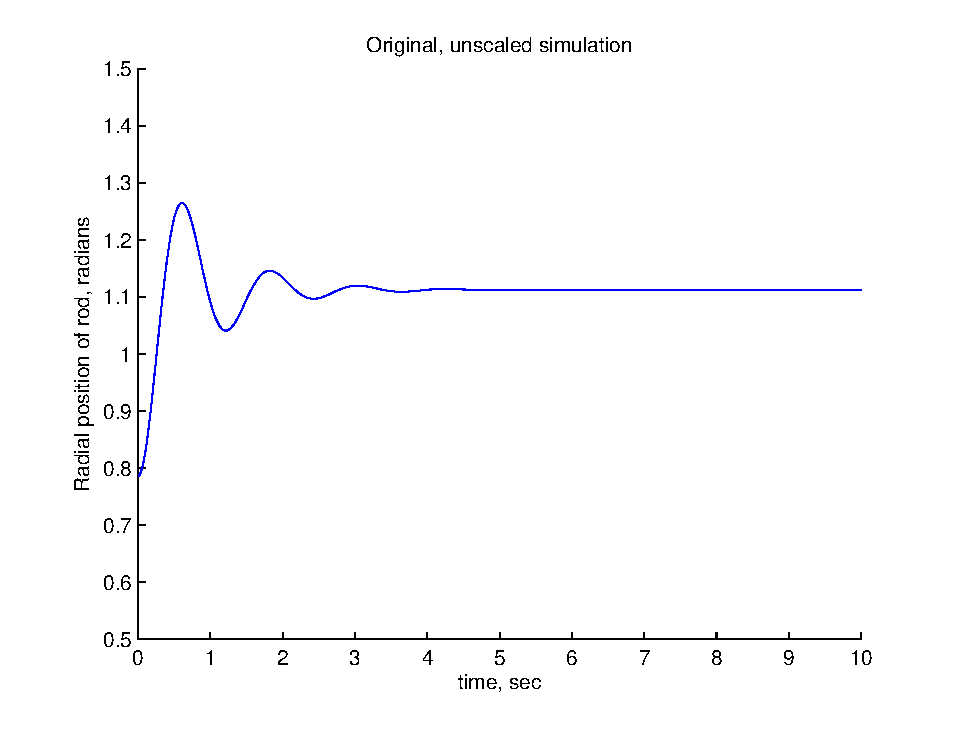
\includegraphics[width=.48\linewidth]{img/original_angular.eps}
  \caption{Original system, no scaling. }
  \label{fig:original_angular}
\end{figure}

\begin{figure}[ht]
  \centering
  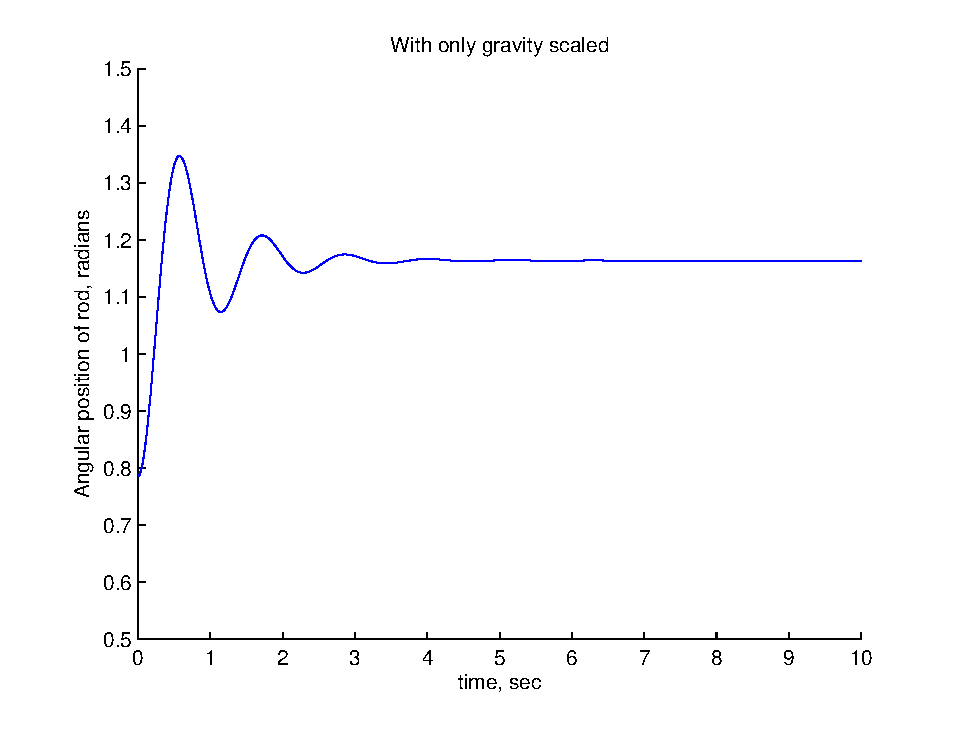
\includegraphics[width=.48\linewidth]{img/grav_only_angular.eps}
  \caption{System with gravity scaled by 2. }
  \label{fig:grav_only_angular}
\end{figure}

\begin{figure}[ht]
  \centering
  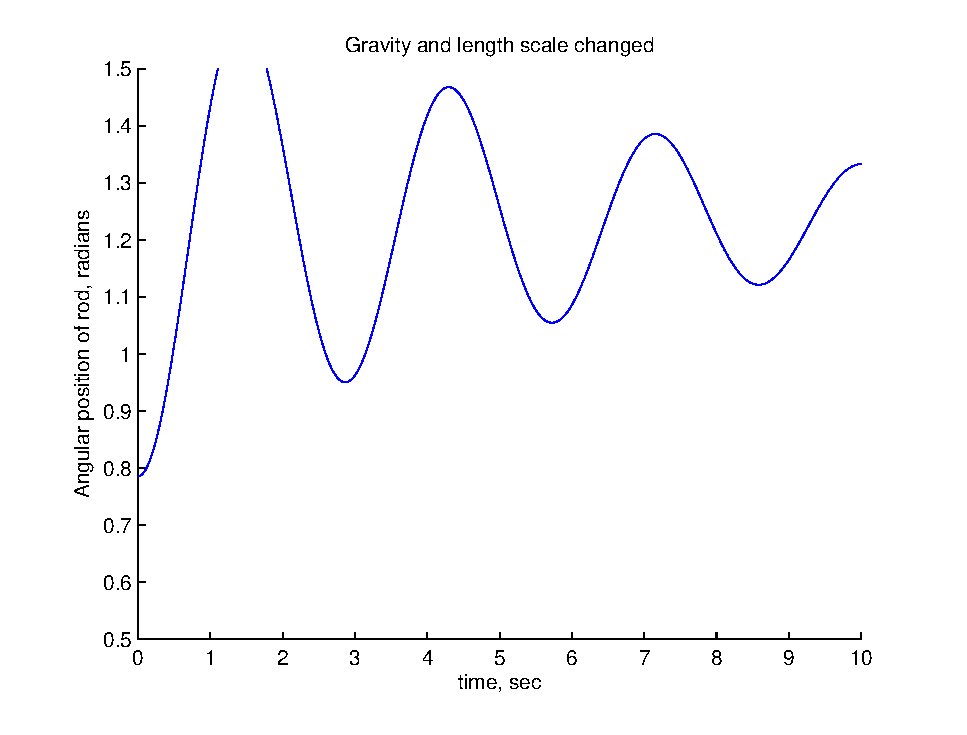
\includegraphics[width=.48\linewidth]{img/l_g_angular.eps}
  \caption{System with length scaled as well as gravity, both proportional with $s$. }
  \label{fig:l_g_angular}
\end{figure}

\begin{figure}[ht]
  \centering
  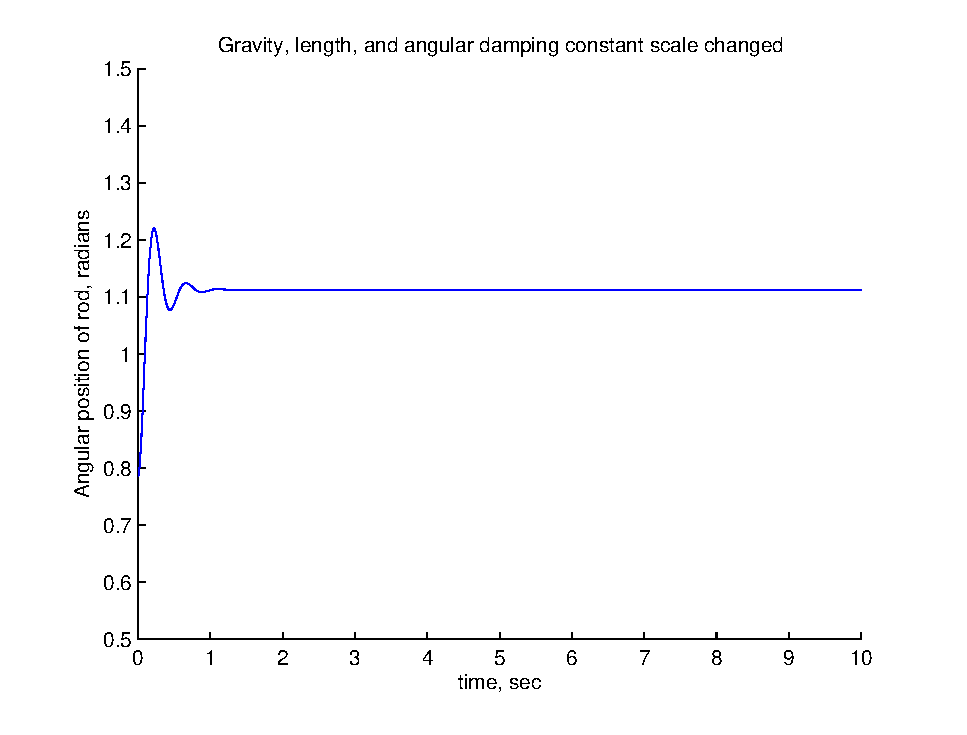
\includegraphics[width=.48\linewidth]{img/l_g_c_angular.eps}
  \caption{System with gravity, angular damping constant, and length scaled. }
  \label{fig:l_g_c_angular}
\end{figure}


What happened? The plots of Figures \ref{fig:grav_only_angular} and \ref{fig:l_g_angular} are wrong, as expected, but so is Figure \ref{fig:l_g_c_angular}!
It's not the same as Figure \ref{fig:original_angular}! 


As designed by this tutorial, plot \ref{fig:l_g_c_angular} shows what happens when not all Pi-terms are calculated or followed.
We're not following the theorem exactly! 
We conveniently left out the Pi-term corresponding to the time scale.
It's possible that this requires scaling also. 
Let's see if including this compels us to change our scalings or to scale additional parameters.
After some algebra, this Pi-term is

\[
\Pi_4 = \Pi_{t} = \frac{t^2 k_{\theta}}{m l^2}
\]

Ack! The time scaling! 
This gets complicated now: ideally, we'd want to find a scaling that doesn't require a change to the time axis - this makes real-time simulations particularly difficult to interpret.
However, a brief bit of investigation leads us to believe that any possible scaling for this system that involves a gravity term will also necessarily involve a time term.
A future task is to show that this is true by either exhaustive search of Pi-term options or by finding other work that would show it as such. 

Here's our final scaling with time:

\[
l_2 = \frac{1}{s} l_1 , \quad \quad c_{\theta_2} = \frac{1}{s} c_{\theta_1}, \quad \quad t_2 = (s) t_1
\]

This system with all four terms scaled is simulated in figure \ref{fig:l_g_c_t_angular}. See how this is the same result as figure \ref{fig:original_angular}, finally!

\begin{figure}[ht]
  \centering
  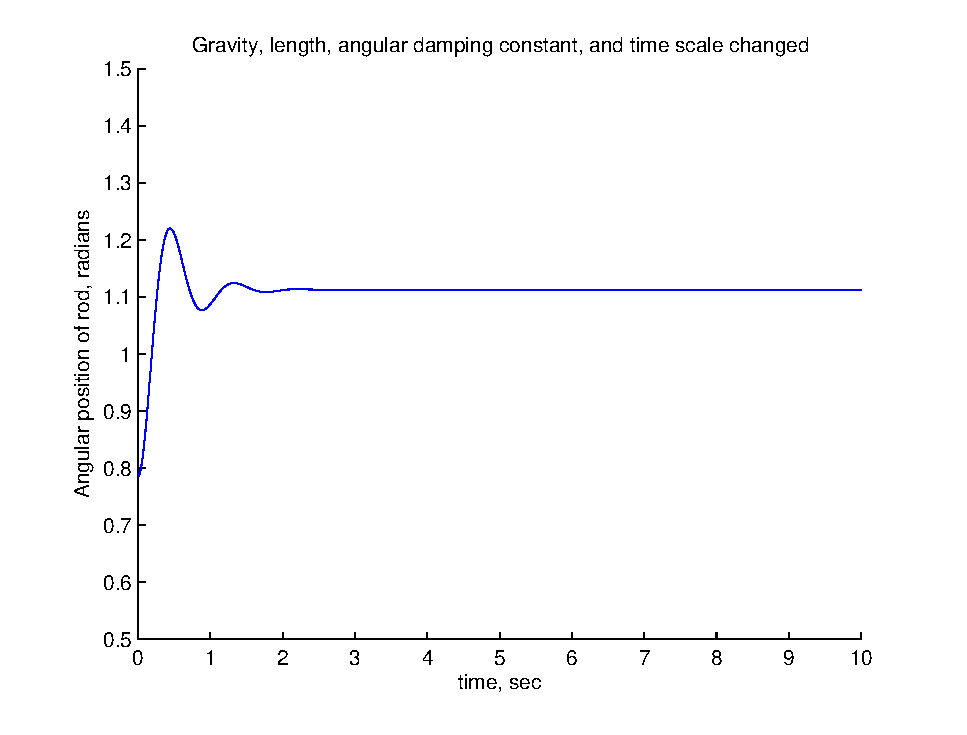
\includegraphics[width=.48\linewidth]{img/l_g_c_t_angular.eps}
  \caption{System with gravity, angular damping constants, and time scaled. }
  \label{fig:l_g_c_t_angular}
\end{figure}

\subsection{Discussion}

This section should show by contradiction that the following two statements are untrue: \\

1. Commutativity of multiplication implies that we only need to scale length when scaling gravity, e.g., only scaling length will result in similitude.
$n * (length / time^2) == (n * length) / time^2.$

If this were true, not only would figures \ref{fig:original_angular} and \ref{fig:l_g_angular} be identical, but there wouldn't be a need for dimensional analysis in the first place.
This conjecture relies on a notion of commutativity of multiplication for a single equation - that involving only length and gravity - and neglects equations that might involve gravity and other terms, or length and other terms.
This is the motivation behind the Buckingham Pi Theorem: such a procedural method ensures that all such interactions are accounted for, and the many potential multiplicative commutativity relationships are always satisfied.

2. Instead of simulating a robot of characteristic size l, mass m and gravity g, we simulate a robot of size 10*l, mass m and gravity 10*g.
The result will be dynamically and kinematically similar (in the technical sense of similitude.)

Similar to the above reasoning, this neglects other possible variables in the system. 
While it is true that such a scaling is needed, this conjecture doesn't consider other possibly-necessary scalings.
In particular, even something like mass may need to be scaled here depending on the situation and if the Pi-terms call for it.
Care must be taken!
However, note again that this does work for certain linear systems, such as those described with the simpler Pi-terms in section 

\section{Analysis of related longitudinal spring/damper systems, for NTRT use}

The above analysis is based on a system where parameters are angular.
However, our simulated systems use longitudinal/linear dampers and springs, along with some other parameters, not angular systems.
The analysis changes quite a bit here!
This is somewhat unexpected at first - why would the units of these extra parameters influence the required scaling for unrelated terms? - but by the Pi theorem, it must work this way.
As alluded to below, this change in scaling requirements arises from the inclusion of a spring constant term that does not depend on length. \\

Ignoring a full dynamics derivation (no more simulations for me!), let's take the following constitutive equations for longitudinal springs and dampers:

\[
F_s = k(x - x_r), \quad F_d = c \dot x
\]

Here are the units of all the CONFIG parameters for the most recent SUPERball model in NTRT.

\[
\text{gravitational acceleration:} \quad g \sim L^1 T^{-2}
\]
\[
\text{density:} \quad \rho \sim M^1 L^{-3}
\]
\[
\text{linear spring rest length:} \quad x_r \sim L^1
\]
\[
\text{linear spring constant:} \quad k \sim M^1 T^{-2}
\]
\[
\text{linear damping coefficient:} \quad c \sim M^1 T^{-1}
\]
\[
\text{pretension force:} \quad F \sim M^1 L^1 T^{-2}
\]
\[
\text{target actuator velocity:} \quad v \sim L^1 T^{-1}
\]
\[
\text{time:} \quad t \sim T^1
\]

Additionally, some models in NTRTsim have other parameters, such as Brian Mirletz' Corde model that uses a shear modulus and modulus of elasticity:

\[
\text{shear modulus:} \quad G \sim M^1 L^{-1} T^{-2}
\]
\[
\text{modulus of elasticity:} \quad E \sim M^1 L^{-1} T^{-2}
\]

Note the missing length scale in $k$ and $c$. 
This is because, for example, $k$ needs to be units of $N/m$ instead of $N/rad$, and the extra length term cancels out.
The new Pi terms, using the same set of $\{m,l,k\}$ are:

\[
\Pi_1 = \Pi_{x_r} = \frac{x_r}{l}
\]
\[
\Pi_2 = \Pi_{g} = \frac{gm}{kl}
\]
\[
\Pi_3 = \Pi_{c} = \frac{km}{c^2}
\]
\[
\Pi_4 = \Pi_{F} = \frac{F}{kl}
\]
\[
\Pi_5 = \Pi_{t} = \frac{t^{2}k}{m}
\]
\[
\Pi_6 = \Pi_G = \frac{Gl}{k}
\]
\[
\Pi_7 = \Pi_E = \frac{El}{k}
\]
\[
\Pi_8 = \Pi_v = \frac{v^2 m}{l^2 d}
\]
\[
\Pi_9 = \Pi_{\rho} = \frac{\rho l^3}{m}
\]

Note that here, the scaling of gravity with length does satisfy almost all of these Pi terms.
When $g$ is multiplied by $s$, we can do the same to $l$.
That then would require scaling by $s$ to $F$ and $v$, scaling by $1/s$ to $G$ and $E$, and by $1/l^3$ to $\rho$.
So, time does not need to be scaled here, but still, five other parameters beyond just gravitational acceleration need to be scaled.
The takeaway here is that without extra Pi terms for more parameters like $k_{\theta}$, we can get away with this simple scaling, but we need to be careful and re-evaluate our Pi terms each time a new unit parameter is introduced.

\section{Scaling Analysis for General Linear Systems}

Finally, I'll finish with an informal argument as to why a truly linear system would not need any of this scaling analysis.
In brief, if input forces can be represented as time-invariant, and the Laplace transform of the system shows a scale of the input to correspond proportionally to an output magnitude change, then scaling is simple and intuitive.
I originally tried these simulations using a simple spring-mass-damper vertically oriented under gravity, e.g.

\[
m \ddot x + c \dot x + k x = mg
\]

With this system, the ''gravity proportional to length'' scaling also works, but for an entirely different reason.
What's actually going on in this case is a change in the magnitude of the input-output transfer function, and so the scaling ITSELF is non-dimensional!
One way to see this is to notice that the gravitational force is time-invariant, and could thus be replaced by a step input:

\[
m \ddot x + c \dot x + k x = u(t)
\]

By superposition of linear systems, the magnitude of the output of the system of

\[
m \ddot x + c \dot x + k x = (n) u(t)
\]

...will be exactly $n$ times larger. Thus, dividing the output by $n$ re-scales to the proper dimensions.
This is, however, informal: more research must be done to show this result, and to review the literature for similar work or proofs.

\section{Moving Forward}

So, after all this work, what should a simulation user do? 

First, review one's model and ensure that the model's scalings are appropriate.
If your model parameters only have the units above, then following the corresponding Pi terms I derived should be enough.
However, if your model either does not include a linear spring constant $k$ or involves other terms not analyzed here, you must do a new dimensional analysis for your results to be correct (e.g. dynamically similar.)

Additionally, simulation users must be mindful of parameters with units inside their controllers, not just in their models.
The Buckingham Pi Theorem only works if all terms in the entire system equations are taken into account, and with a closed-loop controller, the controller dynamics must be included.
As one example, developing a model-based controller with parameters calculated analytically would have to be scaled. 
A controller using nonlinear damping techniques would require a complete re-derivation of these Pi terms and scaling.

Please feel free to use the MATLAB code in the subdirectory here to help analyze your system, if needed. Email me if you find issues.

\bibliographystyle{plain}
\bibliography{scaling_analysis}

\end{document}

% to add?
% a variety of rigid body simulation scalings:
% - air resistance
% - frictional coefficients
% - torsional springs/dampers
% - terms inside controllers: gains? A-Bk?

% To Do before NTRTsim v1.1 release:
% - Move sections around (make this document flow better)
% - Include more justification and explanation, see Ken's email
% - Include scaling analyses for ALL terms in NTRT right now, and hopefully, show at least one of them to violate the ``only l and g'' phenomenon.
